\chapter{Limitations and Future Work}
\label{limitations-chapter}
While request trees provide a~way to evaluate the~transitive consequences of request blocking, the~approach has limitations. Many of the~issues are discussed in previous chapters in their respective sections. This chapter highlights additional limitations not previously addressed and discusses possible future work that could improve the~evaluation process.

\section{Page Behavior That Changes When Content-Blocking Tool Is Present}
\label{page-behavior-unknown}
The method of replaying observed requests and checking which ones are blocked by a~given content-blocking tool does not correctly capture how an~actual page would behave. It assumes that blocking the~requests does not impact the~page's behavior. However, in a~real scenario, the~presence of the~content-blocking tool during a~page visit could influence how the~page responds. For example, if a~request is blocked, the~page might detect the~failure and load the~resource from another source. This blocking could lead to a~different request, possibly with the~same fingerprinting API calls as the~blocked original request. The~current evaluation does not consider this and assumes nothing else follows if a~request is blocked.

This dynamic behavior is impossible to capture for a~deterministic evaluation,  which requires a~fixed dataset, as even if a~content-blocking tool were present during the~logging visit, another tool would behave differently. Since the~dataset cannot account for every possible situation, this issue cannot be resolved.


\section{Limitations of Tree-Based Request Modeling in the~Presence of Cyclic Dependencies}
\label{request_tree_issues}
Throughout the~thesis, the~request structure was referred to as a~\emph{request tree}. However, in practice, the~structure of resources that load on a~web page is not always a~directed tree. Instead, it can form a~regular directed graph that includes loops. For example, a~page may load three scripts \emph{A, B} and \emph{C}. However, each script may re-request the~other scripts. The~situation may look as follows, with requests ordered chronologically:

\begin{itemize}
     \setlength\itemsep{0em}
    \item The~initial page \emph{Z} requests scripts \textit{A} and \textit{B}.
    \item Script \emph{B} requests script \emph{A}, even though it has already been loaded.
    \item Script \emph{A} requests script \emph{C}.
    \item Script \emph{A} requests script \emph{B}, creating a~cycle. 
\end{itemize}

Cycle such as $B \rightarrow A~\rightarrow B$ may execute $1$ to $n$ times, depending on how the~scripts invoke one another. But even if it executes only once, the~resulting requests still constitute a~loop within the~graph. Figure~\ref{request_tree_cycle} illustrates this situation. The~proposed approach cannot correctly capture these cycles.

\begin{figure}[!ht]
    \centering
    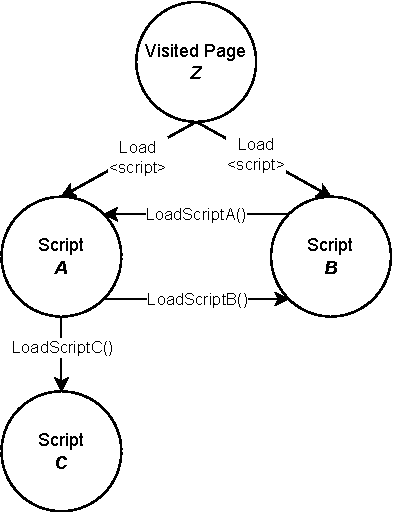
\includegraphics[scale=1]{obrazky-figures/request_tree_cycle.pdf}
    \caption[Request structure graph which is not a~tree]{Example of a~request structure containing a~cycle, which makes it a~directed graph that is not a~tree.}
    \label{request_tree_cycle}
\end{figure}


\subsection{Duplicating Nodes to Ensure Tree Structure}

The proposed evaluation method transforms the~structure into a~tree by introducing duplicate nodes to handle the~loop scenario depicted in Figure~\ref{request_tree_cycle}. This strategy, referred to as the \emph{upper bound} approach, was used to evaluate and compare the selected tools as presented in Chapter \ref{chapter-6}. However, it overestimates the~number of requests, fingerprinting API calls, and possible blocking results. Each valid event in the~logs results in a~new node, even if it is a~duplicate of an~already existing node\footnote{As mentioned in Subsection \ref{req-tree-sub1}, the~exceptions are duplicate follow-up requests loaded by the~same parent (i.e., when page \emph{Z} loads the resource \emph{Y} \emph{n} times, only one copy of \emph{Y} is preserved). These requests are not included in the~\emph{upper bound} approach as keeping them would further worsen the~issues described in this Section.}.

For example, in the~situation described in the~list at the~beginning of this section and captured in Figure~\ref{request_tree_cycle}, script \emph{A} appears twice. Once as a~direct child of the~page and once as a~child of script \emph{B}. Similarly, script \emph{B} also appears twice, as a~direct child of the~page and as a~child of script \emph{A}. Suppose the~script \emph{B} calls a~function from script \emph{A} that leads to requesting script \emph{C}. Script \emph{C} appears only once in the~logs, but it is assigned two parents -- both instances of script \emph{A}, as both were already present in the~tree and the~current approach does not differentiate between them. Figure~\ref{request_tree_cycle_solved} shows the~graph transformed to tree.

\begin{figure}[!ht]
    \centering
    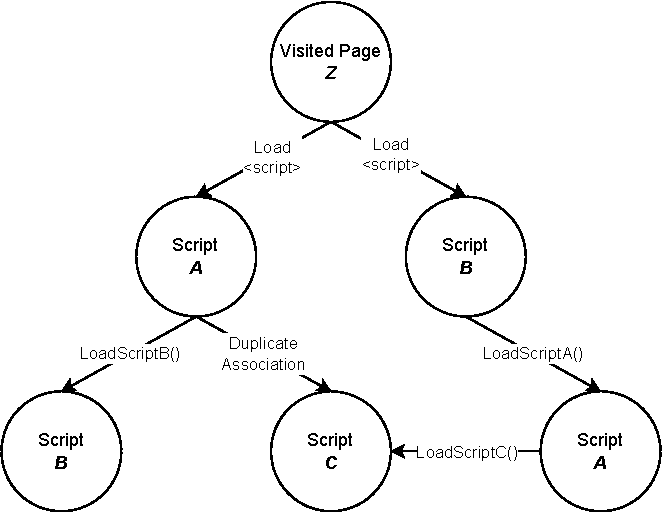
\includegraphics[scale=1]{obrazky-figures/request_tree_cycle_solved.pdf}
    \caption[Resolved loop in the~request structure]{Transformed request structure from Figure \ref{request_tree_cycle} with resolved loop by introducing duplicate nodes, ensuring the~structure is a~tree. Script \emph{C} is present only once, as only a~single network request for it exists. However, as it has two parent scripts \emph{A}, during the~evaluation, it is counted as if it was present twice due to the~tree traversal method.}
    \label{request_tree_cycle_solved}
\end{figure}

\subsection{Node Duplication Overestimates Requests}
The duplication causes the~overestimation of observed requests and possible blocking results. In Figure~\ref{request_tree_cycle_solved}, script \emph{C}, although requested only once, is effectively counted twice, as it is linked to two different parent nodes. Should a~duplicated node be blocked, although it correctly represents two separate requests, the~blocking results might get distorted due to the~duplicated child requests. Also, if script \emph{A} in Figure~\ref{request_tree_cycle_solved} is directly blocked, the~analysis engine blocks both instances, and their child nodes are blocked transitively. As such, the~analysis engine would mark one instance of script \emph{B} as blocked, even though it would still be present on the~page as a~child of the~root node representing the~page itself.

However, the~main issue lies within script \emph{C}. Therefore, the~analysis engine handles it more carefully. Since it is linked to both copies of script \emph{A}, it is only transitively blocked if all of its parent nodes are blocked. All nodes with multiple parent nodes are only transitively blocked if all their parents are blocked. Despite this logic, if script \emph{C} is blocked, it is still incorrectly counted as two blocked requests, which distorts the~results.

\subsection{Impact on Measurements of Access to Fingerprinting APIs}
Another consequence of node duplication is the~distortion of total fingerprinting API calls. The~fingerprinting API calls are assigned to all corresponding nodes -- for example, if script \emph{A} is responsible for $100$ fingerprinting API calls, both instances are assigned $100$ API calls, resulting in $200$ API calls in total.

The duplication is necessary as it is unclear which instance of script \emph{A} was responsible for the~fingerprinting API calls. For example, when script \emph{B} requested script \emph{A}, it may have caused script \emph{A} to call $100$ fingerprinting APIs, while the~root node requesting script \emph{A} did not cause it to use any. Suppose the~traffic parser assigned the~API calls to only one instance, and that particular node was blocked. In that case, it might be wrongly assumed that all fingerprinting API calls caused by script \emph{A} were either entirely prevented or not prevented at all, depending on the~assignment. The~\emph{upper bound} approach assigns them to all copies to avoid underestimating prevented fingerprinting API calls.

\subsection{Avoiding Duplicate Requests}
The request loops are not common. A~\textit{lower bound} approach can be used, which allows each resource to appear only once in the~tree. If the~same script is requested multiple times, the~traffic parser includes only the~first instance in the~request tree. If an~existing node appears multiple times in the~logs, the~traffic parser marks it as \emph{repeated}. Should a~\emph{repeated} node be blocked, the~evaluation would not transitively block any of its child nodes, as blocking them could lead to overestimating the~effectiveness in terms of blocked potential fingerprinting API calls.

\begin{figure}[!ht]
    \centering
    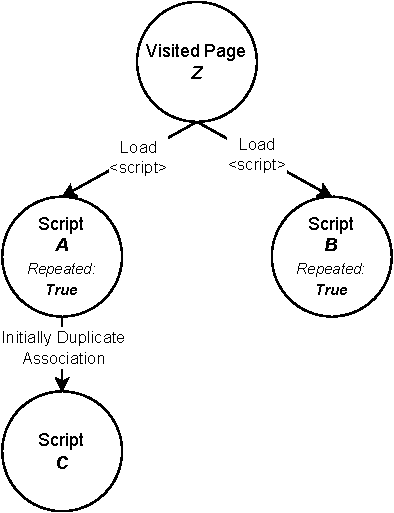
\includegraphics[scale=1]{obrazky-figures/request_tree_lower_bound.pdf}
    \caption[Request tree created using the~\emph{lower bound} approach.]{Request tree created from the~same data as the~tree in Figure~\ref{request_tree_cycle_solved}, but using the~\emph{lower bound} approach. Script \emph{B} requested by script \emph{A} is missing, same as script \emph{A} requested by script \emph{B}. Both remaining instances of \emph{A} and \emph{B} are marked as repeated. Should script \emph{A} be blocked, \emph{C} would not be blocked transitively as its original connection to \emph{A} is missing.}
    \label{request_tree_and_lower_bound}
\end{figure}


Figure~\ref{request_tree_and_lower_bound} illustrates a~request tree created from the~same data as the~request tree shown in Figure~\ref{request_tree_cycle_solved}, but using the~\emph{lower bound} approach. It also explains why the~repeated nodes are not blocked in this approach. Since the~events are parsed chronologically and the~\emph{lower bound} approach does not allow duplicates, the~copy of script \emph{B} requested by script \emph{A} is missing, same as the~copy of script \emph{A} that was initially requested by script \emph{B}.

As a~result, the~missing instance of script \emph{A} never gets the~opportunity to request script \emph{C} and make it call any fingerprinting APIs. Script \emph{C} is still in the~tree because it is connected to the~other instance of script \emph{A}, and that instance is marked as repeated. However, since their association was originally only a~duplicate, it could not have been responsible for any fingerprinting API calls. However, the~calls are still associated with the~script \emph{C}. But since script \emph{A} is marked as repeated, if it were blocked, none of its children would be transitively blocked, keeping the~number of blocked fingerprinting calls caused by script \emph{C} as zero.

Additional limitation of the~\emph{lower bound} approach is, that it discards valid but repeated requests, as seen with scripts \emph{A} and \emph{B} in Figure~\ref{request_tree_and_lower_bound}. Therefore, their associations are lost since each script is only associated with its first parent. For example, if script \emph{A} loads \emph{B} but \emph{B} is already in the~tree as a~child of the~original page, the~relation between \emph{A} and \emph{B} is not created. If script \emph{A} is then blocked, its link to \emph{B} is ignored, even if this instance of \emph{B} made fingerprinting API calls caused by \emph{A}. The~reason why the~request trees do not reflect the~missing parentage is to avoid cycles. For instance, if script \emph{A} loads script \emph{B}, which then loads \emph{A} again, it would introduce a~cycle and break the~logic of the~trees.


\subsection{Summary and Comparison}
Table~\ref{upper_lower_table} compares the~results of both the~\emph{lower} and the~\emph{upper bound} approaches in terms of observed requests and Fingerprinting API calls. Solving the~described problems would require using a~different internal request model that correctly captures all relations between requests without creating duplicates or endless cycles.

\begin{table}[H]
    \centering
    \begin{tabular}{p{21em}|>{\raggedleft\arraybackslash}p{5.2em}|>{\raggedleft\arraybackslash}p{5.2em}}
        \hline
        \multirow{2}{*}{\centering{Total Metric}} &
        \multicolumn{1}{>{\centering\arraybackslash}p{7em}|}{{Lower Bound Approach}} & 
        \multicolumn{1}{>{\centering\arraybackslash}p{7em}}{{Upper Bound Approach}} \\ 
        \hline
 Observed Requests             & 98,244 & 100,753  \\
 \hline
 Browser Properties Fingerprinting API Calls            & 293,498   & 307,226     \\
 Algorithmic Methods Fingerprinting API Calls            & 15,048   & 16,011      \\
 Crawl Fp Inspector Fingerprinting API Calls            & 6,706   & 7,460     \\

        \hline
    \end{tabular}
    \caption[Comparison of total observed requests and fingerprinting API calls in the~dataset between the~\textit{lower} and \emph{upper bound} approaches]{Comparison of total observed requests and fingerprinting API calls in the~dataset between the~\textit{lower} and \emph{upper bound} approaches. The~number of observed requests and fingerprinting API calls is the~same for all tested tools, as they were tested on the~same data, depending on whether the~\textit{lower} or \emph{upper bound} approach was used.}
    \label{upper_lower_table}
\end{table}



\section{Simulation Limitations}
\label{section-of-simulation-limits}
The way the~simulation is designed introduces several limitations. First limitation concerns request schemes and the~other limitation concerns the~functionality of the~tested content-blocking tools. The~issues are challenging to solve, as replicating the~environment of the~original pages from which the~traffic logger collected the~dataset would be required.

\subsection{Request Schemes}
\label{request-schemes-issue}
Many web pages use \textit{data}\footnote{\url{https://developer.mozilla.org/en-US/docs/Web/URI/Reference/Schemes/data}} and \textit{blob}\footnote{\url{https://www.w3.org/TR/FileAPI/\#url}} URL schemes. These schemes behave uniquely and introduce complications during the~evaluation.

In the~case of \textit{blob} scheme, the~issue is that such resources can only be accessed from the~same domain on which they were created\footnote{\url{https://www.w3.org/TR/FileAPI/\#url}}. Thus, if a~custom server requests a~\textit{blob} from another origin, it fails to load, returning an~error. However, on the~original page where the~traffic logger observed the~request, it may have either loaded successfully or been blocked by a~content-blocking tool. Since the~custom server does not replicate the~exact environment of the~original page, it cannot correctly reflect whether a~given content-blocking would block this request, as the~request fails before any blocking can occur. In Firefox, an~additional issue stems from the~fact that the~failed \textit{blob} requests do not trigger the~\texttt{onSendHeaders} event from the~\textit{webRequest} API. As such, the~custom logging extension described in Section~\ref{custom_logging_extension_label} always considers the~\textit{blob} requests blocked, even though it is not necessarily true.

The \textit{data} scheme presents another issue, as these requests do not generate actual network requests to the~Internet. Therefore, they do not trigger the~\texttt{onSendHeaders} event either, and the~custom Firefox logging extension always considers them blocked, even though that may not be the~case, same as the~\textit{blob} requests.

To solve the~described issues, the~current approach in Firefox skips the~\emph{blob} and \emph{data} requests during evaluation, i.e., they are always considered successfully loaded. While this partially solves the~problem, it does not capture the~situation where a~content-blocking tool would have blocked these requests. Firefox logging would need to be improved to handle these situations correctly. The~\textit{blob} scheme problem is unsolvable with the~current approach since these requests will always fail as they cannot be loaded from different domains.

\subsection{Resource Fetching}
\label{simulation_limits}
The other limitation concerns the~method the~simulation loads the~observed resources. During the~simulation, resources are loaded using \texttt{fetch()} API. However, this approach may cause some requests to be blocked or allowed incorrectly because the~simulation engine made them under conditions different from those on an~actual page. For instance, a~content-blocking tool may rely on internal heuristics that decide to block a~request in the~simulated environment, even though it would have been allowed during an~actual page load. There is also the~possibility that some tools detect they are being tested in a~simulated setting and change their behavior.

Another issue stems from the~fact that some content-blocking tools apply rules that block requests based on whether the~requests originate from a~first or third-party context\footnote{\url{https://github.com/gorhill/ublock/wiki/Dynamic-filtering:-rule-syntax}}. Since the~simulation makes requests from a~custom server, these rules are not applicable. 

The issues with resource fetching can distort the~evaluation results. For example, the~tested tool may falsely block a~root node. As discussed in Subsection~\ref{root-results-blocking}, the~analysis engine counts all requests on a~page as blocked if a~requested root node were blocked, even though it might have loaded correctly in an~actual visit.


\section{Future Work}
The issues presented in the~thesis could be quantified based on how much they impact the~results to improve the~evaluation. Once better understood, the~limitations could be addressed to ensure results are more closely aligned with the~real-world behavior of the~evaluated tools. 

The dataset creation process could be optimized to utilize parallelization, as visiting each site one by one takes considerable time. Data collection and the~construction of request models could also be improved to handle the~issues described in Section~\ref{request_tree_issues} properly. Enhancing the~JShelter Fingerprint Detector could also solve the~logging issues described in Subsection~\ref{jshelter-custom-section}, ensuring complete and accurate fingerprinting data collection across all sites. The~simulation could be enhanced to replicate the~environment of the~original pages, which could solve the~limitations of dynamic filters, heuristics and the~\textit{blob} scheme, described in Section~\ref{section-of-simulation-limits}.

Beyond dataset creation, other parts of the~evaluation could also be optimized for parallel execution, which would be especially beneficial when working with large datasets or multiple tools. Only Firefox, Google Chrome, and Chromium-based custom browsers are currently supported. Support for other browsers could be added. New deterministic metrics could also be introduced to analyze different aspects of content-blocking tools. Additionally, the~current metrics could be studied further to understand tool behavior and performance better. Finally, future evaluations could also examine the~broader impact of the~tools, for example, whether they disrupt website functionality or affect page load times.
